\documentclass{article}
\usepackage[utf8]{inputenc}
\usepackage{graphicx}
\usepackage[hidelinks]{hyperref}
\usepackage{hyperref}
\usepackage{graphicx}
\usepackage{subcaption}
\usepackage{float}
\hypersetup{
	colorlinks=false,
	pdfborder={0 0 0},
}


\title{Rendu Final de Projet APS}
\author{Haotian XUE \\ Hejun CAO}
\date{\today}

\begin{document}
	
	\maketitle
	
	\section{Introduction}
	Dans ce projet, nous devons maîtriser les connaissances nécessaires pour créer un nouveau langage, construire des arbres syntaxiques, effectuer la vérification des types ainsi que la vérification sémantique. Le projet est divisé en quatre versions : APS0, APS1, APS1a et APS2. Chaque nouvelle version vise à enrichir les fonctionnalités de la version précédente.
	
	\section{Installation}
	Afin d'exécuter la détection du projet de langage APS, nous devons exécuter le langage de script, saisir chmod +x ./result* dans le terminal Linux et exécuter l'entrée ./resutlAPS\{number\}.sh.
	\begin{figure}[h]
		\centering
		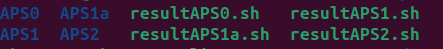
\includegraphics[width=0.8\textwidth]{./images/installation.png}
		\caption{Le dossier principale}
		\label{fig:exemple1}
	\end{figure}
	
	\section{Progression}
	\subsection*{APS0}
	APS0 comprend les opérations de base et les définitions de la langue APS, y compris les opérations arithmétiques telles que l'addition, la soustraction, la multiplication, la division, ainsi que les opérations sur les valeurs booléennes.

	\subsubsection*{Syntaxe :}
	 	ast.ml : ok , parser.mly : ok , lexer.mll : ok
	
	\subsubsection*{Typage :} 
	L'analyse commence à partir du type de prog vers l'intérieur et revient finalement à prog. Si le type de retour est nul, la vérification est réussie.
	\newline \newline
		(PROG)(DEFS)(END)(CONST)(FUN)(FUNREC)(ECHO)(NUM)(ID)(IF)(AND)(OR)(APP)(ABS):ok
	
	\subsubsection*{Sémantique :}
	Utilisez 42 comme résultat de la vérification. Si l'ECHO final est 42, la vérification est réussie.
	\newline \newline
	(PROG)(DEFS)(END)(CONST)(FUN)(FUNREC)(ECHO)(NUM)(ID)(IF)(AND)(OR)(APP)(ABS):ok
	
		\subsection*{APS1}
	APS1 ajoute deux nouveaux conteneurs, Mémoire et Flux, basés sur l'environnement. Mémoire est utilisé pour stocker les adresses, tandis que Flux est utilisé pour mettre à jour et afficher les résultats.
	
	\subsubsection*{Syntaxe :}
	ast.ml : ok , parser.mly : ok , lexer.mll : ok
	
	\subsubsection*{Typage :} 
	(VAR)(PROC)(PROCREC)(SET)(WHILE)(CALL): ok
	
	\subsubsection*{Sémantique :}
	(VAR)(PROC)(PROCREC)(SET)(WHILE)(CALL): ok
	
	\subsection*{APS1a}

	L'extension APS1a à APS1 a été motivée par deux problèmes liés à la gestion des types dans APS1 : premièrement, certains programmes syntaxiquement corrects et bien typés peuvent tout de même causer des erreurs à l'exécution ; deuxièmement, le système de typage dans APS1 ne permet pas la définition de procédures qui modifient leurs arguments
	
	\subsubsection*{Syntaxe :}
	ast.ml : ok , parser.mly : ok , lexer.mll : ok
	
	\subsubsection*{Typage :} 
	(VAR) (SET) (REF) (VAL) (IDV) (IDR) : ok 
	\subsubsection*{Sémantique :}

	(VAR) (SET) (REF) (VAL) (IDV) (IDR) : ok
	
	\subsection*{APS2}
	APS2 continue de se développer sur la base d'APS1a, en ajoutant les opérations len, nth, alloc, vset et autres du tableau ainsi que les types vec.
	
	\subsubsection*{Syntaxe :}
	ast.ml : ok , parser.mly : ok , lexer.mll : ok
	
	\subsubsection*{Typage :} 
	(ALLOC)	(NTH) (LEN)	(VSET) : ok
	
	\subsubsection*{Sémantique :}
	(ALLOC) (NTH) (LEN) (VSET) : ok
	

	
	\section{Implémentation}
	
	\begin{itemize}
		\begin{figure}[H]
			\centering
			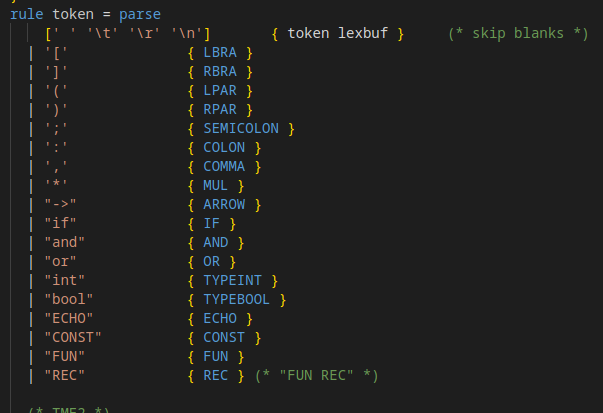
\includegraphics[width=0.8\textwidth]{./images/lexer.png}
			\label{fig:exemple1}
		\end{figure}
	
		\item Définir l'identifiant du jeton du symbole de base.
	
		\begin{figure}[H]
			\centering
			\begin{subfigure}{0.45\textwidth}
				\centering
				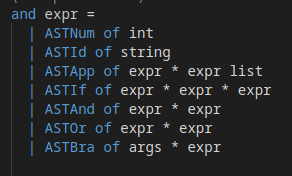
\includegraphics[width=\textwidth]{./images/ast.png} 
				\label{fig:sub1}
				\caption{ast.ml}
			\end{subfigure}
			\hfill
			\begin{subfigure}{0.45\textwidth}
				\centering
				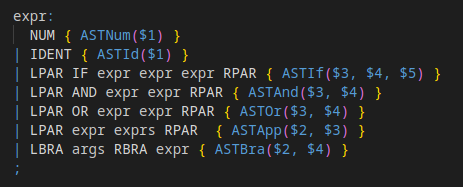
\includegraphics[width=\textwidth]{./images/parser.png} 
				\label{fig:sub2}
				\caption{parser.mly}
			\end{subfigure}
			\label{fig:images}
		\end{figure}
		
		\item Prétraitez le type d'arborescence syntaxique et AST défini dans ast.ml avec le type de jeton défini par parser.mly. Après préparation, utilisez prologTerm pour imprimer la déclaration.
		
		\begin{figure}[H]
			\centering
			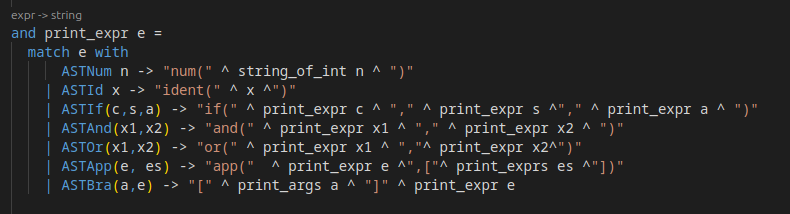
\includegraphics[width=0.8\textwidth]{./images/prologTerm.png}
			\label{fig:exemple1}
		\end{figure}
	
		\item Réorganisez et imprimez tout le contenu avec une sémantique définie dans le terminal.
		
		\begin{figure}[H]
		\centering
		\begin{subfigure}{0.45\textwidth}
			\centering
			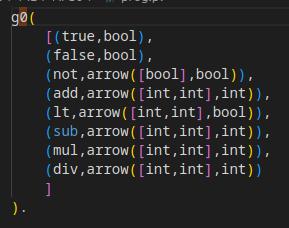
\includegraphics[width=\textwidth]{./images/typage1.png} 
			\label{fig:sub1}
		\end{subfigure}
		\hfill
		\begin{subfigure}{0.45\textwidth}
			\centering
			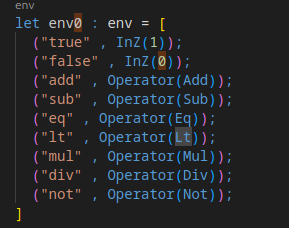
\includegraphics[width=\textwidth]{./images/eval1.png} 
			\label{fig:sub2}
		\end{subfigure}
		\label{fig:images}
		\end{figure}
	
		\item Initialiser l'environnement env0
		
		\begin{figure}[H]
			\centering
			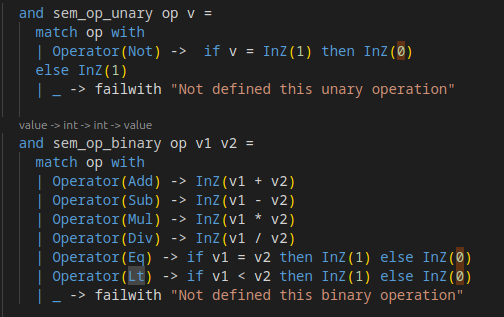
\includegraphics[width=0.8\textwidth]{./images/eval2.png}
			\label{fig:exemple1}
		\end{figure}
		
		\item Opérateurs unaires et binaires séparés
		
		\begin{figure}[H]
			\centering
			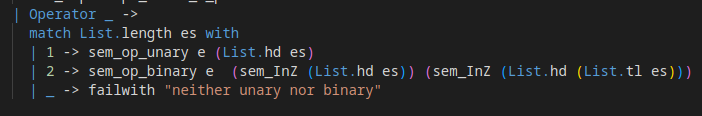
\includegraphics[width=0.8\textwidth]{./images/eval3.png}
			\label{fig:exemple1}
		\end{figure}
		
		\item Rematch des opérateurs séparés
		
		\begin{figure}[H]
			\centering
			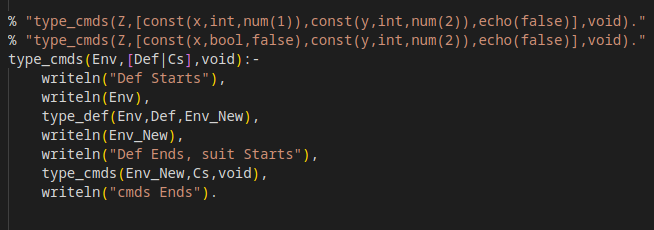
\includegraphics[width=0.8\textwidth]{./images/typage2.png}
			\label{fig:exemple1}
		\end{figure}
		
		\item Lorsque nous rencontrons une erreur introuvable, nous utilisons la méthode d'impression pour déterminer l'emplacement de l'erreur et la déboguer manuellement.
		
		\begin{figure}[H]
			\centering
			\begin{subfigure}{0.45\textwidth}
				\centering
				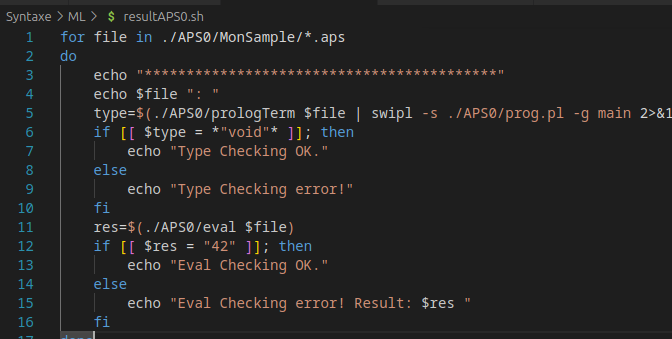
\includegraphics[width=\textwidth]{./images/script.png} 
				\label{fig:sub1}
			\end{subfigure}
			\hfill
			\begin{subfigure}{0.45\textwidth}
				\centering
				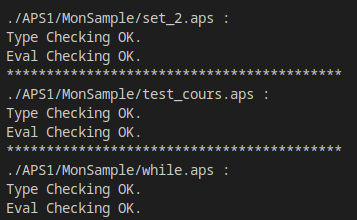
\includegraphics[width=\textwidth]{./images/script2.png} 
				\label{fig:sub2}
			\end{subfigure}
			\label{fig:images}
		\end{figure}
		\item Nous avons mis en pratique un script qui inclut la ligne de commande pour détecter le type et l'évaluation, qui est utilisée pour tester tous les fichiers .aps de MonSample et afficher les résultats sur le terminal.
		
		\item Des fonctions pour implémenter la mémoire: \newline
		1. get\_value (id: string) (env:env) = ... : Trouver la valeur correspondant à l'identifiant dans l'environnement. \newline
		2. mis\_a\_jour id\_list value\_list env = ... : Mettre à jour une liste (id, valeur) dans l'environnement. \newline
		3. getInMem mem adr = ... : Interroger la valeur de l'adresse en mémoire. \newline
		4. newAddress mem = ... : Calculer une nouvelle adresse. \newline
		5. allocMemory mem = ... : Développez une nouvelle mémoire.\newline
		6. replaceElem mem oldElem newElem = ... : Remplacer la valeur existante. \newline
		7. editInMem mem id adr = ... : Remplacer le contenu dans Mem.

			\begin{figure}[H]
			\centering
			\begin{subfigure}{0.45\textwidth}
				\centering
				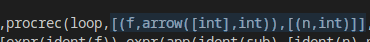
\includegraphics[width=\textwidth]{./images/error.png} 
				\label{fig:sub1}
			\end{subfigure}
			\hfill
			\begin{subfigure}{0.45\textwidth}
				\centering
				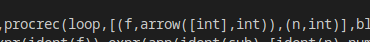
\includegraphics[width=\textwidth]{./images/error_correction.png} 
				\label{fig:sub2}
			\end{subfigure}
			\hfill
			\begin{subfigure}{0.8\textwidth}
				\centering
				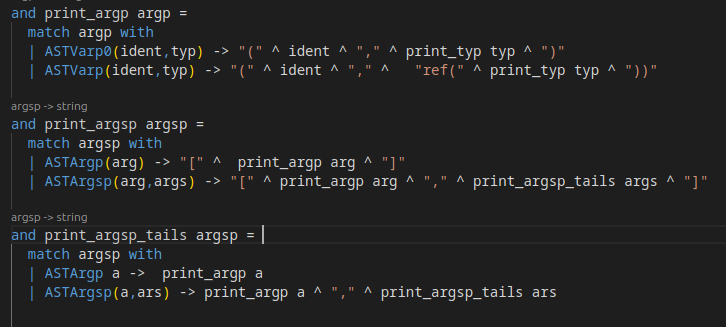
\includegraphics[width=\textwidth]{./images/error_solution.png} 
				\label{fig:sub2}
			\end{subfigure}
			\label{fig:images}
		\end{figure}
		
		\item Nous avons rencontré un problème : [] apparaissait de manière répétée lors des appels récursifs, nous avons donc créé une fonction tail pour éviter ce problème. Faites apparaître [] uniquement au début et à la fin des arguments.

	\end{itemize}


	
\section{Conclusion}

Dans ce projet, nous avons débuté avec les opérations de base et le système de types dans APS0, amélioré la gestion de la mémoire et des flux dans APS1 et APS1a, et finalement supporté des structures de données complexes dans APS2. Chaque version a montré la profondeur et la complexité de la conception des langages de programmation. Ce processus nous a enseigné des techniques clés, allant de la construction des structures de base du langage à l'implémentation de systèmes de types avancés, et à la gestion des erreurs par des tests et du débogage. Le projet a non seulement amélioré nos compétences techniques, mais a aussi renforcé notre capacité à travailler en équipe et à résoudre des problèmes, préparant le terrain pour les défis futurs.

	
	

	
\end{document}
